\noindent V Altiu byla vytvořena DPS pro DP 4. řádu, PP 2. řádu. Keramický vícevrstvý kapacitor byl zvolen vhodný pro pro povrchovou montáž plošných spojů (SMD) 10\,pF, jmenovité napětí stejnosměrného proudu 50\,V, tolerance 10\,\%. \\
\\
Jako zdroj proudu lze použít PNP tranzistor. Řízení OTA vstupním proudem pomocí napěťového zdroje je popsáno na obrázku \ref{s:DC} (Geiger, Sanchez-Sinencio \cite{25}). Toto zapojení je velmi citilivé na malé změny napětí. Z tohoto důvodu je v praktickém zapojení je zvolen přeladitelný odpor. \\
\\
K řízení odporu byl použit přeladitelný odpor o hodnotě 1\,M$\Omega$. Zapojení se zdrojem na 1\,V odpovídá klidový stejnosměrný pracovní proud 1\,$\upmu$A, který odpovídá dvojnásobku proudu použitého v simulaci. Dle dokumentace k simulačnímu bloku LM13700 je reálný proud dvakrát větší. Přeladitelný odpor byl zvolen 3361S-1-105GLF (tolerance 10\,\%, jmenovitý výkon 500\,mW). 
\begin{figure}[h]
\centering
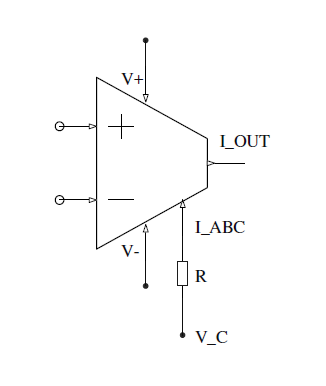
\includegraphics[scale=0.5]{current.png}
\caption{Schéma zapojení napěťového zdroje pro klidový stejnosměrný pracovní proud \label{s:DC}}
\end{figure}
\subsection{Návrhy bikvadů}
\noindent Byly vytvořeny 4 různé návrhy bikvadů. Použito bylo řízení vstupního napětí přeladitelným odporem s PNP tranzistorem, další přeladitelné odpory na doladění mezního kmitočtu jsou u každého OTA. K řízení bylo použito PNP tranzistorové pole s 3 tranzistory v pouzdře. Výstup dolní/pásmová propust lze zvolit přepínačem.\\
\noindent PNP pole bylo zvoleno MMPQ3906, přepínač EG1215AA a EG1315AA, přeladitelný odpor Bourns 3361S.